Tuy nhiên, sử dụng RAG đơn giản
thì độ chính xác chưa cao
và vẫn có thể sai sót
vì vậy,
em sử dụng LangGraph
xây dựng Agentic RAG
để tăng độ chính xác
và hạn chế ảo giác
vì miền tư vấn pháp luật
yêu cầu độ chính xác cao.
% \end{block}
Thay vì thực thi các bước theo quy trình tuyến tính như LangChain, LangGraph mô hình hóa luồng công việc dưới dạng một đồ thị gồm các thành phần chính sau:

\begin{itemize}

\item Nodes (Nút): Đại diện cho các bước xử lý, tác vụ hoặc hành động cụ thể, chẳng hạn như gọi mô hình ngôn ngữ lớn (LLM), truy xuất CSDL hoặc tương tác với người dùng.
\item Edges (Cạnh): Xác định hướng chuyển tiếp giữa các nút. Các cạnh có thể là đường đi trực tiếp hoặc cạnh có điều kiện (conditional edges), cho phép lựa chọn nhánh thực thi dựa trên kết quả của nút trước đó.
\item Cycles (Vòng lặp): Đây là đặc điểm nổi bật của LangGraph. Khác với kiến trúc đồ thị có hướng không chu trình, LangGraph cho phép tác nhân (agent) quay lại các nút đã thực hiện để đánh giá lại kết quả, tự sửa lỗi hoặc lặp lại quy trình nhiều lần cho đến khi đạt được mục tiêu mong muốn.
\item State (Trạng thái): Đây là bộ nhớ dùng chung. Mọi nút (node) trong đồ thị đều có thể đọc dữ liệu từ State này và ghi kết quả mới của chúng vào đây.
\end{itemize}

\begin{figure}[H]
\centering
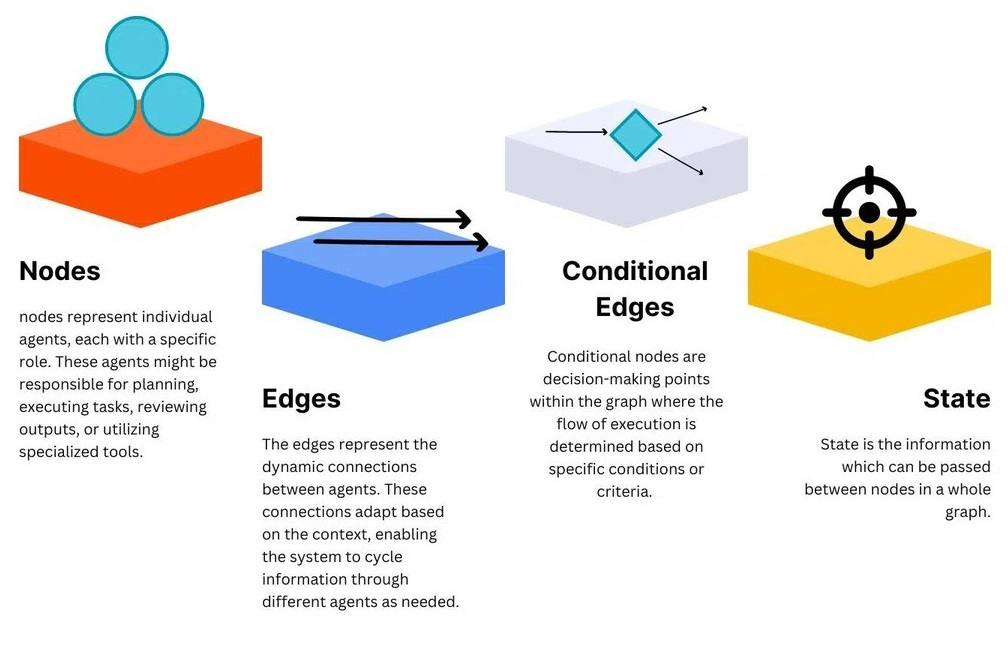
\includegraphics[scale = 0.5]{pictures/625723062_18126048418556935_1835132745978934341_n.jpg}
\caption[Các khái niệm quan trọng của LangGraph]{Các khái niệm quan trọng của LangGraph (Nguồn: \cite{langgraph-innovation})}
\end{figure}

Sơ đồ Agentic RAG dự án này:

\begin{figure}[H]
\centering
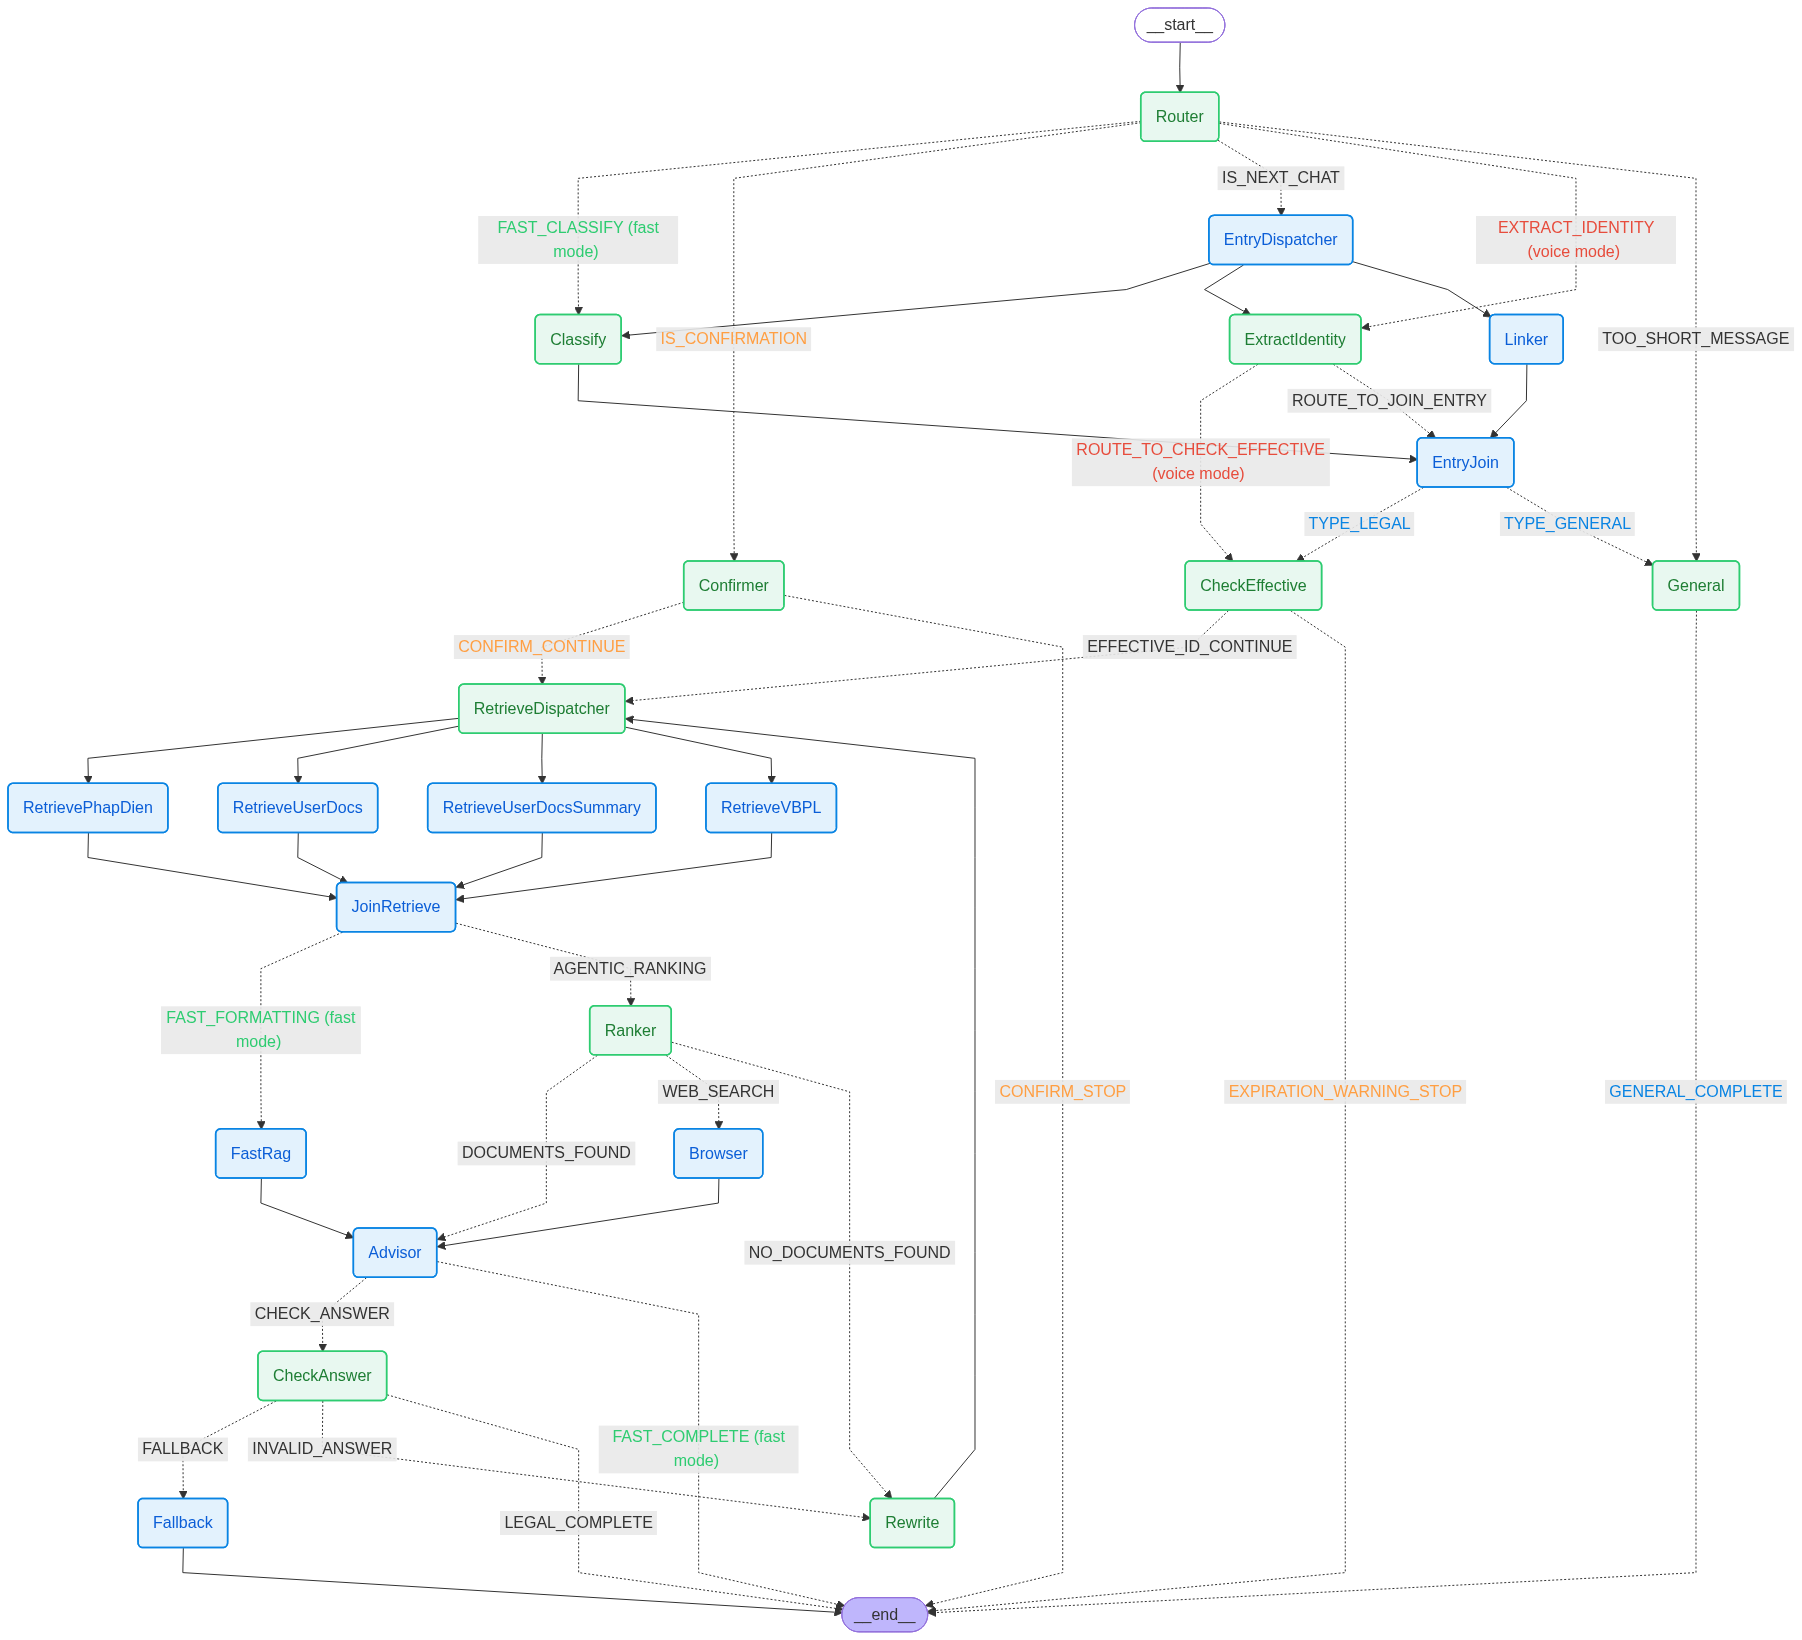
\includegraphics[scale = 0.23]{pictures/rag_diagram.png}
\caption{Sơ đồ LangGraph của dự án}
\end{figure}

Giải thích sơ đồ Agentic RAG:

\begin{itemize}
\item Hệ thống
phân chia việc sử dụng thông minh
giữa mô hình nhỏ cho luồng cơ bản
và mô hình lớn cho tác vụ suy luận
là chìa khóa để tối ưu cả chi phí, độ trễ và hiệu năng.
(Nhìn vào sơ đồ các Node màu xanh lá sử dụng mô hình nhỏ,
các Node màu xanh dương sử dụng mô hình lớn)

\item Mỗi tin nhắn đều đi qua \texttt{Router}.
Node này kiểm tra điều kiện
giúp định tuyến vào luồng chính xác
theo từng trạng thái.

\item Ở chế độ suy luận Agentic RAG đầy đủ
thực hiện
phân tích song song

\begin{itemize}

\item \texttt{Linker} đọc URL nếu có.
\item \texttt{Classify} phân loại câu hỏi là pháp lý hay thông thường.
\item \texttt{Extract Identity} trích xuất số hiệu văn bản (VD: \texttt{100/2019/NĐ-CP}).

\end{itemize}

\item Kiểm tra hiệu lực pháp lý:
Nếu câu hỏi thuộc nhóm \texttt{TYPE\_LEGAL} và có số hiệu văn bản,
hệ thống tra cứu trạng thái.

\begin{itemize}

\item Nếu văn bản đã hết hiệu lực hoàn toàn
thì kết thúc ngay.
\item Nếu văn bản hết hiệu lực một phần
thì phát cảnh báo và chờ người dùng xác nhận ở lượt sau qua \texttt{Confirmer}.

\end{itemize}

% \item Dịch và mở rộng câu hỏi: Trước khi tiến hành truy xuất từ các nguồn dữ liệu, tại nút \texttt{Retrieve Dispatcher}, hệ thống sẽ thực hiện bước dịch câu hỏi nếu đây là lượt chạy đầu tiên. Bước này giúp chuyển đổi các cụm từ mang tính giao tiếp thông thường của người dùng (ví dụ: "sinh viên đi làm thêm") thành các thuật ngữ pháp lý chuyên ngành tương đương (ví dụ: "người lao động thời vụ", "lao động dưới 3 tháng", "thu nhập từ tiền lương tiền công", "giảm trừ gia cảnh") nhằm tối ưu hóa khả năng tìm kiếm trong cơ sở dữ liệu Vector.

\item Truy xuất nguồn dữ liệu song song:
\begin{itemize}
\item Tài liệu người dùng (Milvus)
\item Tóm tắt tài liệu (Cloudflare R2)
\item Văn bản pháp luật (Pinecone)
\item Dữ liệu Pháp Điển (Qdrant)
\end{itemize}

\item Tiếp tục tới \texttt{Ranker} để lọc tài liệu:
\begin{itemize}
\item Nếu có tài liệu hợp lý thì chuyển đến \texttt{Advisor} để tiến hành tạo câu trả lời.
\item Nếu không có tài liệu hợp lý thì chuyển đến \texttt{Rewrite} để tạo lại câu hỏi.
\item Sau khi thử tạo lại câu hỏi vẫn không có tài liệu hợp lý thì sẽ dùng \texttt{Browser} để lấy tài liệu trực tiếp từ các nguồn trực tuyến (thuvienphapluat.vn và luatvietnam.vn).
\end{itemize}

% \item \textbf{Vòng lặp tự kiểm tra chất lượng và xử lý dự phòng (Fallback):} Sau khi \texttt{Advisor} tạo câu trả lời, nút \texttt{Check Answer} sẽ đánh giá xem câu trả lời có chính xác và bám sát tài liệu hay không:
\item Vòng lặp tự kiểm tra chất lượng:
Sau khi \texttt{Advisor} tạo câu trả lời, nút \texttt{Check Answer} sẽ đánh giá xem câu trả lời có chính xác và bám sát tài liệu hay không:
\begin{itemize}
\item Nếu câu trả lời hợp lệ: Hệ thống kết thúc luồng và trả kết quả cho người dùng.
\item Nếu câu trả lời không hợp lệ và số lần thử lại dưới 2 lần: Hệ thống xóa bỏ câu trả lời không đạt yêu cầu khỏi lịch sử trò chuyện, chuyển sang nút \texttt{Rewrite}.
% để tối ưu hóa lại câu truy vấn và thực hiện lại toàn bộ quy trình truy xuất.
\item Nếu không hợp lệ sau khi đã thử lại 2 lần:
Hệ thống chuyển hướng sang \texttt{Fallback}.
% Hệ thống sẽ tự động chuyển hướng sang nút \texttt{Fallback}.
% Tại đây, mô hình sẽ tạo ra một phản hồi lịch sự để thông báo cho người dùng rằng dựa trên các văn bản pháp luật hiện hành được tra cứu, chưa tìm thấy quy định cụ thể nào trực tiếp giải đáp câu hỏi của họ, đồng thời tóm tắt các thông tin pháp lý chung có liên quan nhất từ ngữ cảnh đã được truy xuất (ví dụ: các chính sách chung về thuế thu nhập cá nhân, mức giảm trừ gia cảnh, hoặc quy định về lao động thời vụ...), giúp tránh tình trạng hệ thống chỉ trả về câu hỏi gốc của người dùng.
\end{itemize}

\item Ở chế độ Fast RAG
chỉ đi qua \texttt{Classify} để phân loại.
Sau đó truy xuất dữ liệu lấy dữ liệu.
Dùng \texttt{Advisor} trả lời
và
hệ thống kết thúc quá trình trả lời
mà không cần bước kiểm tra.

\item Ở chế độ giọng nói Voice,
do đã có Agent nên không cần qua bước phân loại của LangGraph
và người dùng không thể nhập URL nên hệ thống chuyển đến \texttt{Extract Identity} trích xuất số hiệu văn bản.

\end{itemize}
